%%%%%%%%%%%%%%%%%%%%%%%%%%%%%%%%%%%%%%%%%
% Beamer Presentation
% LaTeX Template
% Version 1.0 (10/11/12)
%
% This template has been downloaded from:
% http://www.LaTeXTemplates.com
%
% License:
% CC BY-NC-SA 3.0 (http://creativecommons.org/licenses/by-nc-sa/3.0/)
%
%%%%%%%%%%%%%%%%%%%%%%%%%%%%%%%%%%%%%%%%%

%----------------------------------------------------------------------------------------
%	PACKAGES AND THEMES
%----------------------------------------------------------------------------------------

\documentclass{beamer}

\mode<presentation> {

% The Beamer class comes with a number of default slide themes
% which change the colors and layouts of slides. Below this is a list
% of all the themes, uncomment each in turn to see what they look like.

%\usetheme{default}
%\usetheme{AnnArbor}
%\usetheme{Antibes}
%\usetheme{Bergen}
%\usetheme{Berkeley}
%\usetheme{Berlin}
%\usetheme{Boadilla}
%\usetheme{CambridgeUS}
%\usetheme{Copenhagen}
%\usetheme{Darmstadt}
%\usetheme{Dresden}
%\usetheme{Frankfurt}
%\usetheme{Goettingen}
%\usetheme{Hannover}
%\usetheme{Ilmenau}
%\usetheme{JuanLesPins}
%\usetheme{Luebeck}
\usetheme{Madrid}
%\usetheme{Malmoe}
%\usetheme{Marburg}
%\usetheme{Montpellier}
%\usetheme{PaloAlto}
%\usetheme{Pittsburgh}
%\usetheme{Rochester}
%\usetheme{Singapore}
%\usetheme{Szeged}
%\usetheme{Warsaw}

% As well as themes, the Beamer class has a number of color themes
% for any slide theme. Uncomment each of these in turn to see how it
% changes the colors of your current slide theme.

%\usecolortheme{albatross}
%\usecolortheme{beaver}
%\usecolortheme{beetle}
%\usecolortheme{crane}
%\usecolortheme{dolphin}
%\usecolortheme{dove}
%\usecolortheme{fly}
%\usecolortheme{lily}
%\usecolortheme{orchid}
%\usecolortheme{rose}
%\usecolortheme{seagull}
%\usecolortheme{seahorse}
%\usecolortheme{whale}
%\usecolortheme{wolverine}

%\setbeamertemplate{footline} % To remove the footer line in all slides uncomment this line
%\setbeamertemplate{footline}[page number] % To replace the footer line in all slides with a simple slide count uncomment this line

%\setbeamertemplate{navigation symbols}{} % To remove the navigation symbols from the bottom of all slides uncomment this line
}

\usepackage{graphicx} % Allows including images
\usepackage{booktabs} % Allows the use of \toprule, \midrule and \bottomrule in tables
\usepackage{listings}
\usepackage{amsmath}
\usepackage{algpseudocode,algorithm,algorithmicx}

\lstdefinestyle{custom}{
  breaklines=true,
  frame=L,
  xleftmargin=\parindent,
  language=Java,
  showstringspaces=false,
  basicstyle=\footnotesize\ttfamily,
  keywordstyle=\ttfamily\bfseries\color{green!40!black},
  commentstyle=\ttfamily\itshape\color{gray!40!black},
  identifierstyle=\color{blue},
  stringstyle=\color{orange},
  tabsize = 2
}

%----------------------------------------------------------------------------------------
%	TITLE PAGE
%----------------------------------------------------------------------------------------

\title[B Trees]{B Trees} % The short title appears at the bottom of every slide, the full title is only on the title page

\author{Jonathan Windle} % Your name
\institute[UEA] % Your institution as it will appear on the bottom of every slide, may be shorthand to save space
{
University of East Anglia \\ % Your institution for the title page
\medskip
\textit{J.Windle@uea.ac.uk} % Your email address
}
\date{\today} % Date, can be changed to a custom date

\begin{document}

\begin{frame}
\titlepage % Print the title page as the first slide
\end{frame}

\begin{frame}[allowframebreaks]
\frametitle{Overview} % Table of contents slide, comment this block out to remove it
\tableofcontents % Throughout your presentation, if you choose to use \section{} and \subsection{} commands, these will automatically be printed on this slide as an overview of your presentation
\end{frame} 

%------------------------------------------------------------------
\section{Intro}
\begin{frame}
\frametitle{Intro}
\begin{itemize}
\item Let $K$ be a totally ordered set.
\item A {\color{red} 2-3 tree}, $t$ is a tree on $K \cup (K \times K)$ possessing the following properties:
\begin{itemize}
\item Each non-leaf node has {\color{green} 2 or 3 children}
\item If $p$ is a node with 2 children then it contains one key sych that:
\begin{itemize}
\item All keys in the left subtree of $p < key(p) <$ all keys in the right subtree of $p$.
\end{itemize}
\item If $p$ is a node with 3 children, then it contains two keys, $ltkey$ and $rtkey$, such that:
\begin{itemize}
\item All keys in the left subtree of $p$:
\item $< ltkey$
\item $<$ all keys in the middle subtree of $p$
\item $< rtkey$
\item $<$ all keys in right subtree of $p$.
\end{itemize}
\item All leaf nodes are at the same level.
\end{itemize}
\end{itemize}
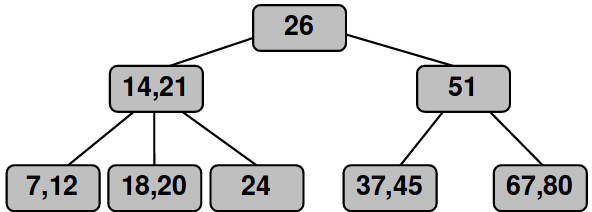
\includegraphics[scale=0.2]{btree.png}
\end{frame}

%----------------------------------------------------------------
\section{Inserting}
\subsection{Inserting - Case 1}
\begin{frame}
\frametitle{Inserting - Case 1}
Insertion in a leaf node containing a single key:\\
E.g. Insert 25:\\
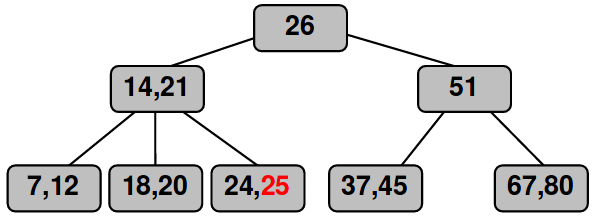
\includegraphics[scale=0.5]{single.png}
\end{frame}
%-------------------------------------------------------------------
\subsection{Inserting - Case 2}
\begin{frame}
\frametitle{Inserting - Case 2}
Node whose children should contain new key has only two children, both with two keys:\\
E.g. Insert 55:\\
\begin{itemize}
\item Go to right child of node containing 51; inserting 55 in this node would give {\color{red}55},{\color{blue}67},80;
\item Make the middle key of these 3 keys the right key of the parent;
\item Split the other two values into two nodes.
\end{itemize}
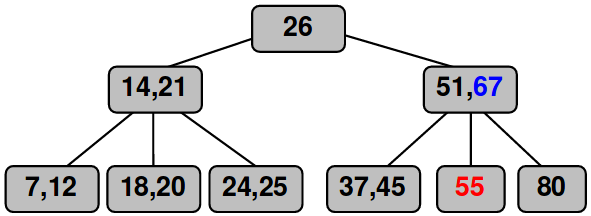
\includegraphics[scale=0.3]{case2.png}
\end{frame}
%------------------------------------------------------------------
\subsection{Inserting - Case 3}
\begin{frame}
\frametitle{Inserting - Case 3}
Node whose children should contain new key already has 3 children, and new key cannot be inserted in a leaf containing just 1 key.\\
E.g. insert 16:\\
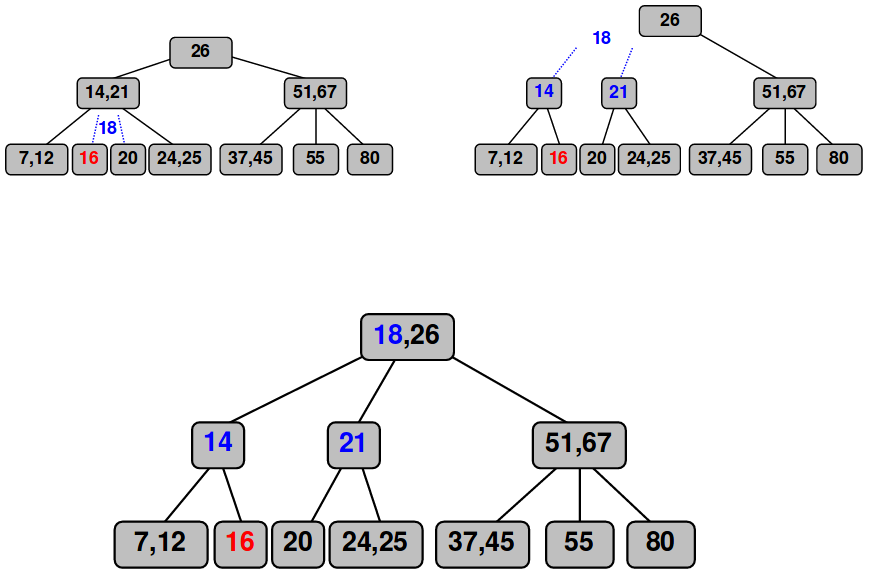
\includegraphics[scale=0.3]{case3.png}
\end{frame}
%-----------------------------------------------------------------
\subsection{Inserting - Case 4}
\begin{frame}
\frametitle{Inserting - Case 4}
Splitting the root\\
E.g. Insert 16 in\\
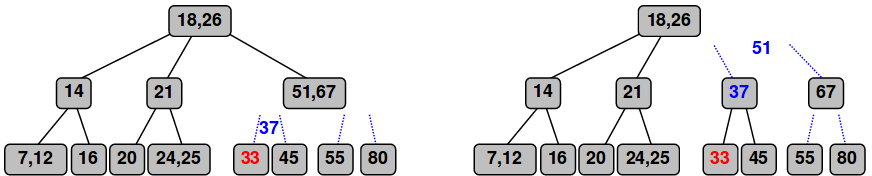
\includegraphics[scale=0.3]{case4-1.png}\\
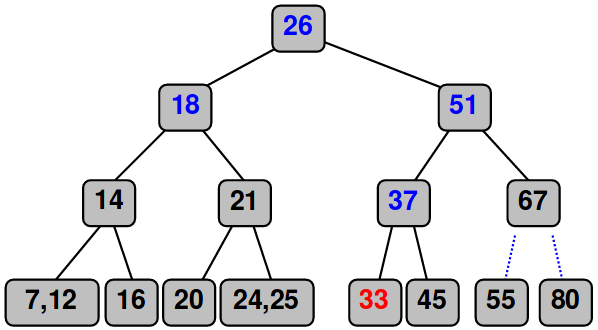
\includegraphics[scale=0.3]{case4-2.png}
\end{frame}
%---------------------------------------------------------------
\section{B-Trees}
\begin{frame}
\frametitle{Intro}
\begin{itemize}
\item A 2-3 tree is a B-Tree of {\color{red} order 3}.
\item More generally,a{\color{green}B-tree of order $m$} is an $m$-way search tree such that:
\begin{itemize}
\item If the root is not a leaf nodethen it has between 2 and $m$ children.
\item All non-leaf nodes except the root have between [$m/2$] and $m$ children.
\item All leaf nodes are at the same level.
\end{itemize}
\item The path length when searching in a B-tree is bounded above by:\\
$log_{[m/2]}(\frac{n+1}{2})$
\end{itemize}
\end{frame}
%---------------------------------------------------------------
\subsection{Comparison}
\begin{frame}
\frametitle{Comparison of Height-Balanced Binary Search Trees and B-Trees}
\begin{itemize}
\item The expected path length  in a height-blances BST containing $n$ keys is:\\
$[log_2(n+1)] - 1$
\item Height of a B-tree of order $m$ containing $n$ keys is:\\
$\leq log_{[m/2]}(\frac{n+1}{2})$.
\item It is easier to code BST algorithms
\item B-Trees waste space if used for RAM-based dictionaries.
\item B-Trees on disk units have $m$ = 256 or more:\\
$shallow \ tree \Rightarrow fewer \ disk \ accesses$
\end{itemize}
\end{frame}
%-----------------------------------------------------------------

\begin{frame} 
\Huge{\centerline{The End}}
\end{frame}

\end{document}